% !TeX spellcheck = en_GB
~
\pagebreak

\section{Standalone version of Hibernate Search}

\begin{figure}[ht]
	\centering
	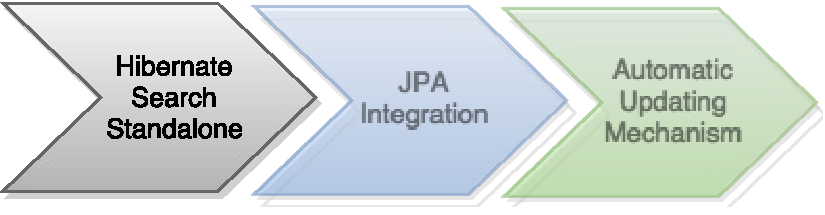
\includegraphics[scale=0.75]{images/timeline_genericjpa_first.pdf}
	\label{project_timeline_first}
\end{figure}
\noindent
We will start the development part of this thesis by discussing how Hibernate Search's engine (in the form of the module "hibernate-search-engine") can be used in general. After this is done we will work out a standalone version of this engine that is easier to work with so we can integrate this standalone version with JPA in the next chapter.
\\\\
As already described earlier (\ref{problem_indexing_searching}), hibernate-search-engine is not intended to be used by application developers, but for other APIs to integrate with. Therefore there is no real public documentation available on how to use it and all following information had to be retrieved from tests in the hibernate-search-engine and hibernate-search-orm integration module source code.

\pagebreak

\subsection{Example project with Hibernate Search annotations} \label{setting_up_example_project}

Before we explain how we do things in particular, we set up the example entities described in \ref{example_project} as if the original Hibernate Search would have been used. We do so by adding additional annotations to our entity-classes:

\begin{enumerate}
	\item \textbf{@Indexed}: marks the entity as an index root-type.
	\item \textbf{@DocumentId}: marks the field as the id of this entity. this is only needed if no JPA @Id can be found, but can be used to override settings.
	\item \textbf{@Field}: describes how the annotated field should be indexed. The fieldname defaults to the Java property name.
	\item \textbf{@IndexedEmbedded}: marks properties that point to other classes which should be included in the index. By default, all fields contained in these entities are prefixed with the property name this is placed on.
	\item \textbf{@ContainedIn}: used in entities that are embedded in other indexes. this is set on the properties that point back to the index-owning entity.
\end{enumerate}
\noindent
As these annotations are defined in hibernate-search-engine, we can rely on all of them while designing the standalone version of Hibernate Search and all other modules depending on it.

\pagebreak
\noindent
The resulting entities look like this:
\\
\lstset{language=java}
\lstset{moredelim=[is][\bfseries]{[*}{*]}}
\begin{lstlisting}[frame=htrbl, caption={Book.java with Hibernate Search annotations}, label={lst:book.java_2}]
@Entity
@Table(name = "Book")
[*@Indexed*]
public class Book {

	@Id
	@Column(name = "isbn")
	[*@DocumentId*]
	private String isbn;
	
	@Column(name = "title")
	[*@Field(store = Store.YES, index = Index.YES)*]
	private String title;
	
	@Column(name = "genre")
	[*@Field(store = Store.YES, index = Index.YES)*]
	private String genre;
	
	@Lob
	@Column(name = "summary")
	[*@Field(store = Store.NO, index = Index.YES)*]
	private String summary;
	
	@ManyToMany(mappedBy = "books", cascade = {
		CascadeType.MERGE,
		CascadeType.DETACH,
		CascadeType.PERSIST,
		CascadeType.REFRESH
	})
	[*@IndexedEmbedded(includeEmbeddedObjectId = true)*]
	private Set<Author> authors;
	
	//getters & setters ...
}
\end{lstlisting}

\pagebreak

\lstset{language=java}
\lstset{moredelim=[is][\bfseries]{[*}{*]}}
\begin{lstlisting}[frame=htrbl, caption={Author.java with Hibernate Search annotations}, label={lst:author.java_2}]
@Entity
@Table(name = "Author")
public class Author {

	@Id
	@GeneratedValue(strategy = GenerationType.AUTO)
	@Column(name = "authorId")
	[*@DocumentId*]
	private Long authorId;
	
	@Column(name = "firstName")
	[*@Field(store = Store.YES, index = Index.YES)*]
	private String firstName;
	
	@Column(name = "lastName")
	[*@Field(store = Store.YES, index = Index.YES)*]
	private String lastName;
	
	@Column(name = "country")
	[*@Field(store = Store.YES, index = Index.YES)*]
	private String country;
	
	@ManyToMany(cascade = {
		CascadeType.MERGE, 
		CascadeType.DETACH, 
		CascadeType.PERSIST, 
		CascadeType.REFRESH
	})
	@JoinTable(name = "Author_Book", 
		joinColumns = 
			@JoinColumn(name = "authorFk", 
				referencedColumnName = "authorId"),
		inverseJoinColumns = 
			@JoinColumn(name = "bookFk", 
				referencedColumnName = "isbn"))
	[*@ContainedIn*]
	private Set<Book> books;
	
	//getters & setters ...
}
\end{lstlisting}

\pagebreak

\subsection{Usage of Hibernate Search's engine} \label{using_hsearch_engine}
In this chapter we will take a look at how to use Hibernate Search's engine natively by showing how it's started, how the index is manipulated and how searching works.

\subsubsection{Startup}
A Hibernate Search engine instance is represented by a \textbf{SearchIntegrator} object. In order to obtain it, we first have to write a special configuration class that implements \textbf{org.hibernate.search.cfg.spi.SearchConfiguration}. An object of this class has then to be created and filled with all the configuration properties Hibernate Search requires. The minimum that has to be set for this to work are the following:

\begin{enumerate}
	\item \textbf{hibernate.search.default.directory\_provider}: The two most common cases here are either "ram" or "filesystem". This decides where the index will be stored. A ram directory is only present in the system memory while the SearchIntegrator exists. A "filesystem" directory is persisted on the hard disk. For "filesystem" the additional property "hibernate.search.default.indexBase" has to be set to an appropriate path.
	
	\item \textbf{hibernate.search.lucene\_version}: This decides which Lucene version has to be used internally. The currently latest supported version is "4.10.4".
\end{enumerate}
\noindent
A complete list of the available settings can be found in the Hibernate Search documentation \footnote{Hibernate Search documentation, see~\cite{hibernate_search_doc}} (only the Hibernate ORM specific settings cannot be used). Our \textbf{StandaloneSearchConfiguration} (appendix listing \ref{lst:StandaloneSearchConfiguration.java}) defaults to "ram" and "4.10.4".
\\\\
Having this class in place, a \textbf{SearchIntegrator} can be obtained by a \textbf{SearchIntegratorBuilder} like this:
\\
\lstset{language=java}
\lstset{moredelim=[is][\bfseries]{[*}{*]}}
\begin{lstlisting}[frame=htrbl, caption={Starting up the engine}, label={lst:starting_up_engine.java}]
List<Class<?>> indexClasses = Arrays.asList(Book.class, Author.class);

SearchConfiguration searchConfiguration = 
	new StandaloneSearchConfiguration();
indexClasses.forEach( searchConfiguration::addClass );

//bootstrapping class for Hibernate Search
SearchIntegratorBuilder builder = new SearchIntegratorBuilder();

//we have to build an integrator here (the builder needs a 
//"base integrator" first before we can add index classes)
builder.configuration( searchConfiguration ).buildSearchIntegrator();

indexClasses.forEach( builder::addClass );

//starts the engine with all configuration properties set
SearchIntegrator searchIntegrator = builder.buildSearchIntegrator();

//use the integrator ...

//close it
searchIntegrator.close();
\end{lstlisting}

\subsubsection{Index manipulation}

Now that we know how a SearchIntegrator can be built, we can take a look at how we can control the index using the engine's features. 
\\\\
The engine does a lot of optimizations in the backend. This is the reason the specifics are hidden behind a \textbf{Worker} pattern. Such a worker batches operations by synchronizing upon the \textbf{org.hibernate.search.backend.TransactionContext} interface. Our implementation of this is simply called \textbf{Transaction} (appendix listing \ref{lst:Transaction.java}). The different index operations are represented by \textbf{Work} objects that contain the WorkType (INDEX, UPDATE, PURGE, etc.) and all necessary data to execute the individual task.
\\\\
Indexing objects with \textbf{WorkType.INDEX}:
\\
\lstset{language=java}
\begin{lstlisting}[frame=htrbl, caption={Indexing an object with the engine}, label={lst:indexing_object_native.java}]
Book book = ...;
Transaction tx = new Transaction();
Worker worker = searchIntegrator.getWorker();
worker.performWork( new Work( book, WorkType.INDEX ), tx );
tx.commit();
\end{lstlisting}

\pagebreak
\noindent
Updating objects with \textbf{WorkType.UPDATE}:
\\
\lstset{language=java}
\begin{lstlisting}[frame=htrbl, caption={Updating an object with the engine}, label={lst:updating_object_native.java}]
Book book = ...;
Transaction tx = new Transaction();
Worker worker = searchIntegrator.getWorker();
worker.performWork( new Work( book, WorkType.UPDATE ), tx );
tx.commit();
\end{lstlisting}
~\\
Deleting objects with \textbf{WorkType.PURGE}:
\\
\lstset{language=java}
\begin{lstlisting}[frame=htrbl, caption={Deleting an object by id with the engine}, label={lst:deleting_object_native.java}]
String isbn = ...;
Transaction tx = new Transaction();
Worker worker = searchIntegrator.getWorker();
worker.performWork( new Work( Book.class, isbn, WorkType.PURGE ), tx );
tx.commit();
\end{lstlisting}
~\\
This API doesn't have any "convenience" methods that wrap around the Transaction management if no batching is needed, nor does it have any wrapper utility for the Work object generation.

\pagebreak

\subsubsection{Queries}
Querying the index is already acceptable to some extent when it comes to building the actual query. This is mainly due to the fact the query class \textbf{HSQuery} supports method chaining and that the same query builder DSL used in Hibernate Search ORM is available (the Builder returns a Lucene query. Any basic Lucene query could be used as well, but require manual analysis of the input. Queries produced by the builder are automatically analysed with the correct Analyzer).
\\
\lstset{language=java}
\lstset{moredelim=[is][\bfseries]{[*}{*]}}
\begin{lstlisting}[frame=htrbl, caption={Querying the index with the engine}, label={lst:querying_natively.java}]
SearchIntegrator searchIntegrator = ...;

HSQuery query = searchIntegrator.createHSQuery();

//find information about all the entities matching a given title
[*List<EntityInfo>*] entityInfos = 
	query.luceneQuery(
			//query DSL:
			searchIntegrator.buildQueryBuilder()
				.forEntity( Book.class )
				.get()
				.keyword()
				.onField( "title" )
				.matching( "searchString" )
				.createQuery()
		).targetedEntities(
			Collections.singletonList(
				Book.class
			)
		)[*.projection(
			ProjectionConstants.ID
		)*].queryEntityInfos();
\end{lstlisting}

\pagebreak
\noindent
The queries don't return anything resembling the original Java objects, though. The actual data returned depends on what we project upon in the projection(...) call and is wrapped in an \textbf{EntityInfo} object. In the example above we only retrieve the ids of the Books matching our query. We do this because when using a search index, we don't generally want to work with the actual data found in the index after the hits have been found. We want objects retrieved from the database.
\\
\lstset{language=java}
\begin{lstlisting}[frame=htrbl, caption={Extracting info from the results}, label={lst:querying_natively.java_2}]
//a JPA EntityManager
EntityManager em = ...;

//extract info from the entityInfos
for(EntityInfo entityInfo : entityInfos) {
	String isbn = (String) entityInfo.getProjection()[0];
	//retrieve an object from the database
	Book book = em.find(Book.class, isbn);
	//handle this information ...
}
\end{lstlisting}

\pagebreak

\subsection{Design of the standalone version} \label{standalone_hibernate_search}

In \ref{using_hsearch_engine} we described how the engine can be used natively without any notion of JPA. While using the engine this way is possible, it is not feasible because some of the code is quite complicated. This is the reason we will now discuss a standalone abstraction of this code.
\\\\
As we have seen in the examples earlier, the main class used for index control and querying are \textbf{SearchIntegrator} and \textbf{HSQuery}. In order to abstract some of the complicated logic, we now introduce two new interfaces: 

\begin{itemize}
	\item \textbf{StandaloneSearchFactory}: This interface is responsible for all index changes. Code using this abstraction doesn't have to cope with the Worker pattern, at all. This is hidden behind index/delete/update methods.
	
	\item \textbf{HSearchQuery}: While still having the same chaining methods as HSQuery, we retrieve results from the index in a different manner now. Instead of manually having to extract the ID out of the EntityInfos, this interface retrieves the actually wanted data with the help of the \textbf{EntityProvider} interface which wraps the access to the database. The specifics of the EntityProvider are still use-case specific as the examples later in this chapter will show.
\end{itemize}

\pagebreak

\noindent
The following diagram shows the rough architecture of our new standalone version. Note that we are using a specialization of \textbf{SearchIntegrator} - namely \textbf{ExtendedSearchIntegrator} - which allows us to have more sophisticated features.
\\
\begin{figure}[ht]
	\centering
	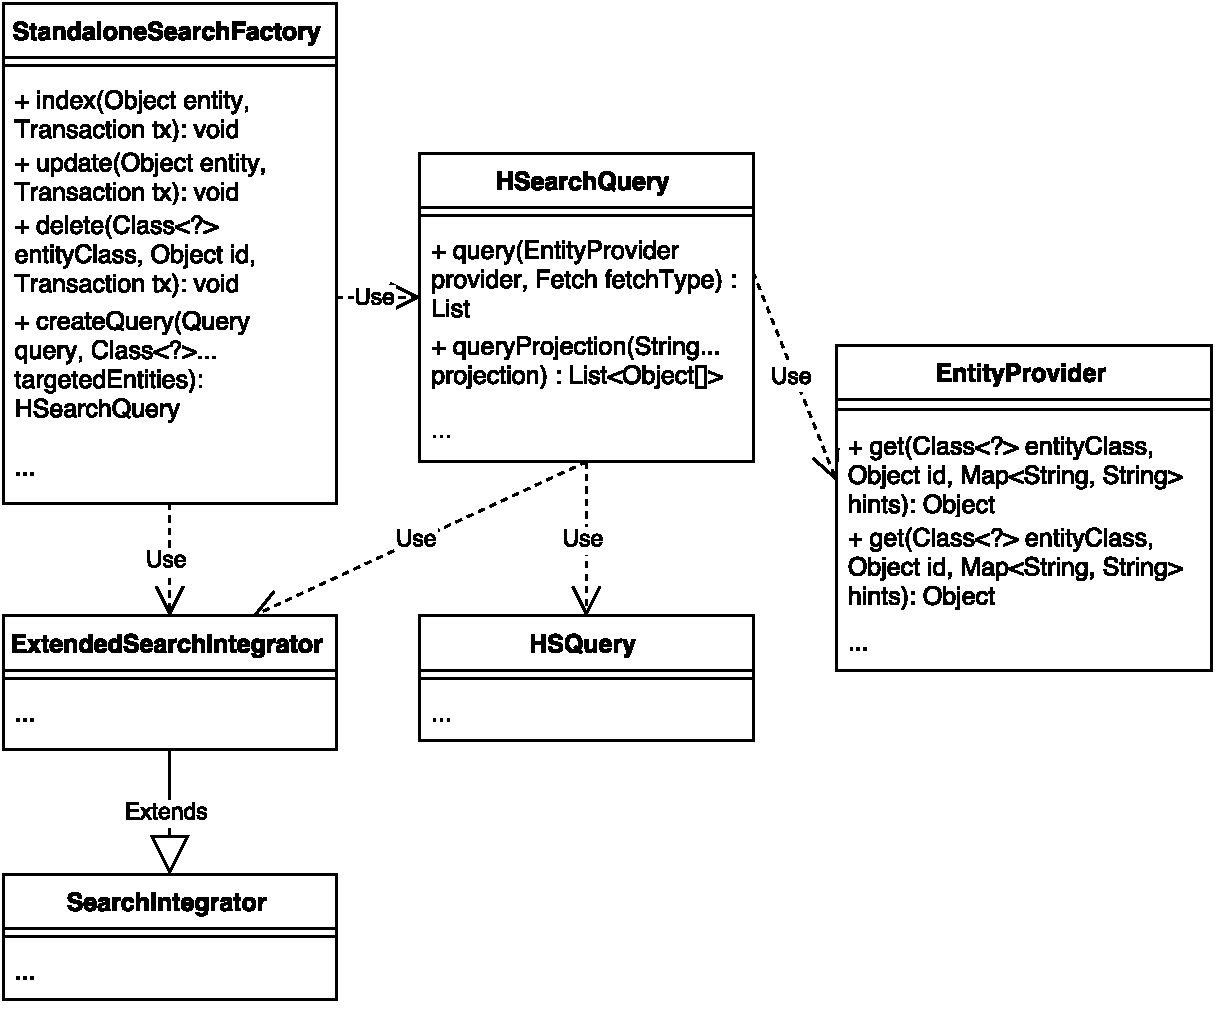
\includegraphics[scale=0.6]{images/standalone_min_architecture.pdf}
	\caption{Rough architecture of the standalone version (important parts)}
	\label{standalone_min_architecture}
\end{figure}

\pagebreak

\subsubsection{Startup}

The startup process of the standalone version doesn't differ much from manually using the engine in terms of configuration as we still have to use the SearchConfiguration interface. The only difference is how we build the StandaloneSearchFactory. This is done with a \textbf{StandaloneSearchFactoryFactory}, so the code using it doesn't have to handle the creation of the actual implementation object.
\\
\lstset{language=java}
\lstset{moredelim=[is][\bfseries]{[*}{*]}}
\begin{lstlisting}[frame=htrbl, caption={Starting up the standalone version}, label={lst:using_standalone.java}]
List<Class<?>> indexClasses = Arrays.asList(Book.class, Author.class);

//we still have to build the SearchConfiguration object
SearchConfiguration searchConfiguration = 
		new StandaloneSearchConfiguration();
indexClasses.forEach( searchConfiguration::addClass );

//the builder pattern from before is abstracted in the following lines
StandaloneSearchFactory searchFactory = 
		StandaloneSearchFactoryFactory.
				createSearchFactory(
					searchConfiguration,
					indexClasses
				);
				
//use the searchfactory ...

//close it
searchFactory.close();
\end{lstlisting}

\pagebreak

\subsubsection{Index manipulation}

With our standalone version, basic index control becomes more streamlined as we don't have to work with  SearchIntegrator's Worker pattern anymore.
\\
\lstset{language=java}
\begin{lstlisting}[frame=htrbl, caption={Indexing an object with the standalone version}, label={lst:indexing_object_native.java}]objects
Book book = ...;
Transaction tx = new Transaction();
searchFactory.index(book, tx);
tx.commit();
\end{lstlisting}

\lstset{language=java}
\begin{lstlisting}[frame=htrbl, caption={Updating an object with the standalone version}, label={lst:updating_object_native.java}]
Book book = ...;
Transaction tx = new Transaction();
searchFactory.update(book, tx);
tx.commit();
\end{lstlisting}

\lstset{language=java}
\begin{lstlisting}[frame=htrbl, caption={Deleting an object by id with the standalone version}, label={lst:deleting_object_native.java}]
Transaction tx = new Transaction();
String isbn = ...;
searchFactory.delete(Book.class, isbn, tx);
tx.commit();
\end{lstlisting}

\pagebreak

\subsubsection{Queries} \label{querying_standalone}
The biggest change in the standalone version is probably how the index is queried. We don't have to work with EntityInfos anymore as we introduced the \textbf{EntityProvider} interface. This interface hosts one method that is to be used for batch fetching (Fetch.BATCH) and one for single fetching (Fetch.FIND\_BY\_ID).
\\\\
A good default implementation delegating the database access to a JPA EntityManager is our \textbf{BasicEntityProvider} (\ref{lst:BasicEntityProvider.java}). Besides taking an EntityManager in its constructor, the class also needs a Map<Class<?>, String> containing the id properties of the entities. While we leave the construction of this map out in the following example for the sake of simplicity, the code for this can be found in the listings (\ref{lst:idProperties.java}). After its creation this map can then be stored in a central place and reused.
\\
\lstset{language=java}
\begin{lstlisting}[frame=htrbl, caption={Querying the index with the standalone version}, label={lst:querying_natively.java}]
StandaloneSearchFactory searchFactory = ...;

EntityManager em = ...;
Map<Class<?>, String> idProperties = ...;

EntityProvider entityProvider = new BasicEntityProvider(em, idProperties);

List<Book> books = searchFactory
			.createQuery(searchFactory.buildQueryBuilder()
				.forEntity(Book.class)
				.get()
				.keyword()
				.onField("title")
				.matching("searchString")
				.createQuery(), Book.class
			).query(
				entityProvider,
				Fetch.BATCH
			);
\end{lstlisting}

\pagebreak

\section{JPA integration of the standalone version} \label{integration_jpa}

\begin{figure}[ht]
	\centering
	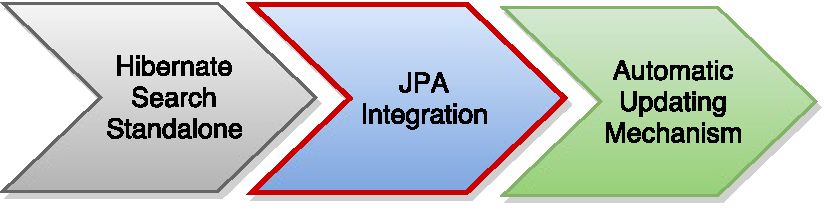
\includegraphics[scale=0.75]{images/timeline_genericjpa_second.pdf}
	\label{project_timeline_second}
\end{figure}
\noindent
After simplifying the access to Hibernate Search's engine we will work out an integration with JPA interfaces next. Since we started with the premise of not wanting to "reinvent the wheel" by writing everything from scratch (as described in \ref{reinvent_the_wheel}) - which was one of the reasons why we chose to use Hibernate Search's engine in the first place - we will try to build an integration as similar to the JPA interfaces of Hibernate Search ORM as possible.
\\\\
Before we can go into detail about how we build our integration, we have to discuss the general architecture first. We will go over how the Hibernate Search ORM integration with JPA interfaces behaves from a user point and then take a look at what has to be changed in order to be compatible with any JPA implementor.

\pagebreak

\subsection{Architecture of Hibernate Search ORM}

Hibernate Search ORM integrates with the JPA API by extending the interfaces  javax.persistence.EntityManager and javax.persistence.Query and adding new functionality to the fulltext search versions of these interfaces: \textbf{FullTextEntityManager} and \textbf{FullTextQuery}. The following figure shows a rough overview of this. Note that this contains only the methods relevant for the following sections.
\\
\begin{figure}[ht]
	\centering
	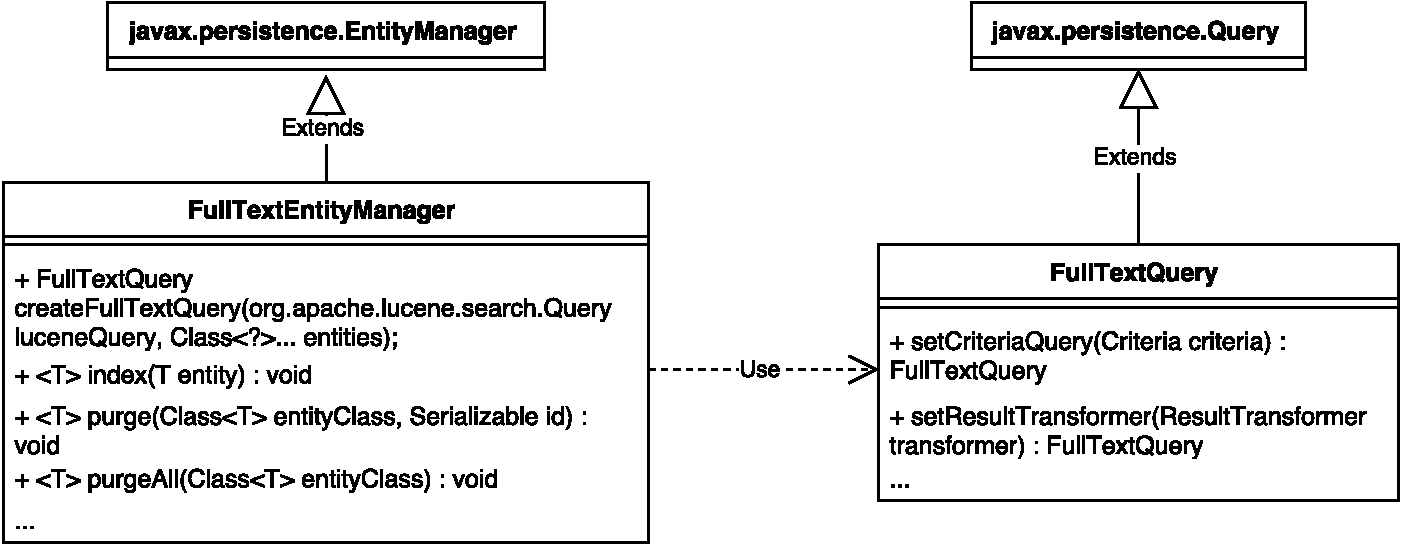
\includegraphics[scale=0.6]{images/hibernate_search_jpa_integration_original.pdf}
	\caption{The main JPA interfaces of Hibernate Search ORM}
	\label{hibernate_search_jpa_integration_original}
\end{figure}

\pagebreak

\subsection{Startup}
As Hibernate Search ORM is tightly coupled with Hibernate ORM it is automatically started if found on the classpath and the persistence.xml contains the following:
\\
\lstset{language=java}
\begin{lstlisting}[frame=htrbl, caption={Additions to persistence.xml with Hibernate Search ORM}, label={lst:hibernate_search_persistence.xml}]
...
<property name="hibernate.search.default.directory_provider"
value="filesystem"/>
<property name="hibernate.search.default.indexBase"
value="/path/to/indexes"/>
...
\end{lstlisting}
\noindent
This means that there exists no real code entry point as Hibernate Search is fully integrated into the Hibernate ORM/OGM lifecycle. FullTextEntityManagers can therefore be obtained with:
\\
\lstset{language=java}
\begin{lstlisting}[frame=htrbl, caption={Obtaining a FullTextEntityManager with Hibernate Search ORM}, label={lst:indexing_object_hsearch_orm_jpa.java}]
EntityManager em = ...;
FullTextEntityManager fem = Search.getFullTextEntityManager(em);
\end{lstlisting}
All of FullTextEntityManager's operations are controlled by the same transactions the original Hibernate EntityManager is using. This is the reason we will not have any search transaction related code in the following paragraphs.

\pagebreak

\subsubsection{Index manipulation}
The index operations are all straightforward and similar to what we designed our standalone version in \ref{standalone_hibernate_search} to work like apart from minor naming differences. 
\\\\
Hibernate Search ORM doesn't differentiate between indexing and updating.
\\
\lstset{language=java}
\begin{lstlisting}[frame=htrbl, caption={Indexing/Updating an object with Hibernate Search ORM}, label={lst:indexing_object_hsearch_orm_jpa.java}]
FullTextEntityManager fem = ...;
Book book = ...;
fem.index(book);
\end{lstlisting}
\noindent
Deleting objects from the index is called purging. This is probably due to not wanting to confuse it with JPA's delete(...).
\\
\lstset{language=java}
\begin{lstlisting}[frame=htrbl, caption={Deleting an object by id with Hibernate Search ORM}, label={lst:deleting_object_hsearch_orm_jpa.java}]
FullTextEntityManager fem = ...;
String isbn = ...;
fem.purge(Book.class, isbn);
\end{lstlisting}

\pagebreak

\subsubsection{Queries} \label{hsearch_orm_querying}
Hibernate Search ORM integrates even better with JPA for queries than our standalone version as the FullTextQuery interfaces extends the JPA Query interface and uses getResultList() to return its results.
\\
\lstset{language=java}
\begin{lstlisting}[frame=htrbl, caption={Querying with Hibernate Search ORM}, label={lst:querying_hsearch_orm.java_1}]
EntityManager em = ...;
FullTextEntityManager fem = Search.getFullTextEntityManager(em);

FullTextQuery fullTextQuery = fem.createFullTextQuery(
	fem.getSearchFactory().buildQueryBuilder()
		.forEntity( Book.class )
		.get()
		.keyword()
		.onField( "title" )
		.matching( "searchString" )
		.createQuery(), 
	Book.class);
	
List<Book> books = (List<Book>) fullTextQuery.getResultList();
\end{lstlisting}

\pagebreak

\subsubsection{Index rebuilds}
A noteworthy feature of Hibernate Search is its MassIndexer. It can be used whenever the way the entities are indexed is changed (e.g. in the @Field annotations). It uses multiple threads working in parallel to scroll results from the database and then indexes these efficiently. This is by far faster than the naive approach working in only one thread. It also incorporates a lot of internal improvements a normal developer wouldn't have access to as the specifics are hidden in the implementation packages of Hibernate Search which are not intended to be used outside of its own code.
\\\\
A full index rebuild for our Book entity would look like this:
\\
\lstset{language=java}
\begin{lstlisting}[frame=htrbl, caption={MassIndexer usage with Hibernate Search ORM}, label={lst:massindexing_hsearch_orm.java}]
EntityManager em = ...;
FullTextEntityManager fem = Search.getFullTextEntityManager(em);

fem.createIndexer( Book.class )
	.batchSizeToLoadObjects( 25 )
	.threadsToLoadObjects( 12 )
	.idFetchSize( 150 )
	.transactionTimeout( 1800 )
	.startAndWait();
\end{lstlisting}
\noindent
"This will rebuild the index of all [Book] instances (and subtypes), and will create 12 parallel threads to load the User instances using batches of 25 objects per query; these same 12 threads will also need to process indexed embedded relations and custom FieldBridges or ClassBridges, to finally output a Lucene document."\footnote{Hibernate Search documentation (MassIndexer, v5.4), see~\cite{hibernate_search_doc_massindexer}}

\pagebreak

\subsection{Architecture of the generic version}

As good as Hibernate Search ORM's API integration with JPA's EntityManager and Query interface is, its additional interfaces still contain some Hibernate ORM related features and logic that a generic version (we call it Hibernate Search GenericJPA) can not support and therefore have to be changed, emulated or removed all together.
\\
\begin{figure}[ht]
	\centering
	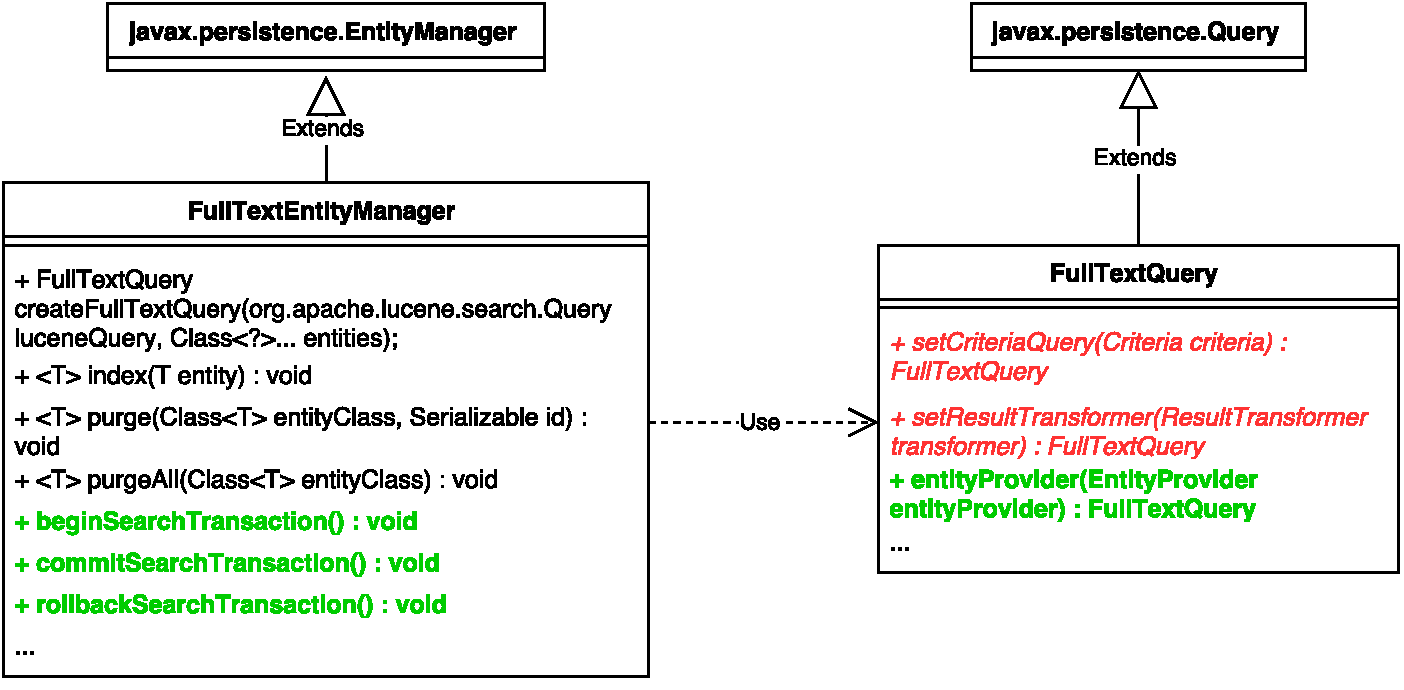
\includegraphics[scale=0.6]{images/hibernate_search_jpa_integration_with_differences.pdf}
	\caption{Required fixes for a generic version}
	\label{hibernate_search_jpa_integration_with_differences}
\end{figure}
\\
In the figure above, we marked all the methods requiring to be fixed in the FullTextEntityManager and FullTextQuery interfaces:
\begin{itemize}
	\item green: new methods
	\item red: methods that can't be supported
	\item olive: methods that can be supported if changed
\end{itemize}
\noindent
Besides these, some other aspects need changes as well. We will discuss all of the needed changes \& additions in the following paragraphs.

\pagebreak

\subsubsection{Startup}

In our generic version we can't tightly integrate with the EntityManagerFactory of the JPA provider. This is the reason we introduce a separate interface called \textbf{JPASearchFactoryController}.

\begin{figure}[ht]
	\centering
	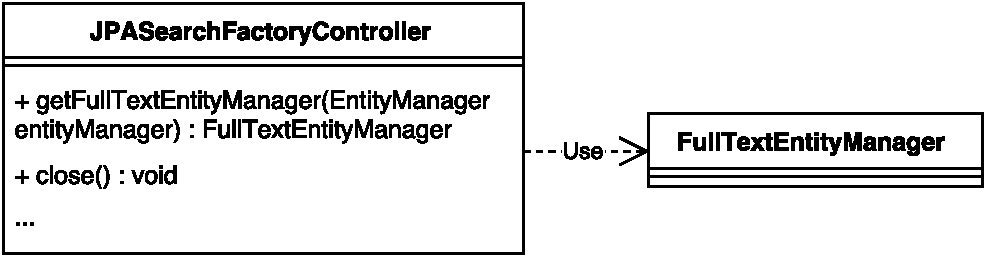
\includegraphics[scale=0.6]{images/JPASearchFactoryController.pdf}
	\caption{JPASearchFactoryController}
	\label{jpa_searchfactory_controller}
\end{figure}
\noindent
Having this separate interface means that its lifecycle has to be controlled on its own.
\\\\
Unlike the static way a FullTextEntityManager is obtained in Hibernate Search ORM via the Search class, in our generic version, we obtain it with the \textbf{getFullTextEntityManager(EntityManager entityManager)} method (the Search class works in Hibernate Search ORM only because of the tight coupling of ORM and Search). This means that an instance of the JPASearchFactoryController has to be available at all times when access to the index is required.
\\\\
Using a non-static approach here has one benefit, though: We can pass null to this method and get a search only FullTextEntityManager that can be used to work on the index when no database access is needed. This is particularly useful if POJOs have to be indexed which are not associated with JPA (see table \ref{table:config_properties_jpasearchfactorycontroller}, property "hibernate.search.additionalIndexedTypes").
\\\\
We start the fulltext search engine with our bootstrapping class \textbf{Setup} like this:
\\
\lstset{language=java}
\begin{lstlisting}[frame=htrbl, caption={MassIndexer usage with Hibernate Search ORM}, label={lst:massindexing_hsearch_orm.java}]
//In Hibernate Search ORM, the fulltext engine would be started 
//together with the EntityManagerFactory.
//In GenericJPA we can't do that.
EntityManagerFactory emf = ...;

EntityManager em = ...;

Properties properties = new Properties();

properties.setProperty(
	"hibernate.search.searchfactory.type", 
	"manual-updates"
);

//In GenericJPA this starts the fulltext engine to 
//which a reference is returned by this method call
JPASearchFactoryController searchFactoryController =
	Setup.createSearchFactoryController( emf, properties );

//FullTextEntityManagers are not obtained with the Search class
FullTextEntityManager fem = 
	searchFactoryController.getFullTextEntityManager(em);

//use it...

searchFactoryController.close();
\end{lstlisting}
\noindent
For this example we are using "manual-updates", as we haven't discussed how the index is kept up-to-date. After we worked that out, "manual-updates" will just be a fallback setting for developers not wanting to have the index automatically updated.  Also note that there are many more properties that can be set and vanilla Hibernate Search settings are passed this way as well. A complete list of the available GenericJPA configuration properties can be found in table \ref{table:config_properties_jpasearchfactorycontroller} in the appendix.

\pagebreak

\subsubsection{Index manipulation} \label{using_hsearch_genericjpa_index}

In Hibernate Search ORM, all manual index manipulation is synchronized with the EntityManager transaction lifecycle (index changes underly the JPA transaction system). In our generic approach we cannot do this as JPA doesn't have an extension point for this kind of usage. This is the reason we introduce the \textbf{[begin/commit/rollback]SearchTransaction()} methods in FullTextEntityManager. These have to be used to control the transaction lifecycle of all the index manipulation methods:
\\
\lstset{language=java}
\begin{lstlisting}[frame=htrbl, caption={Index control with Hibernate Search GenericJPA}, label={lst:index_control_hibernatesearchgenericjpa}]
EntityManager em = ...;
JPASearchFactoryController searchFactoryController = ...;

FullTextEntityManager fem = 
	searchFactoryController.getFullTextEntityManager(em);

fem.beginSearchTransaction();
try {
	//index or purge here
	fem.commitSearchTransaction();
} catch(Exception e) {
	fem.rollbackSearchTransaction();
	throw e;
}
\end{lstlisting}
\noindent
By introducing our own search transaction management methods we don't restrict the usage of GenericJPA in application servers by a lot compared to the original Hibernate Search ORM because manual index changes are not needed frequently. In general these transactions can not be compared with real RDBMS transactions anyways as it is allowed to write changes to the index without commiting with flushToIndexes(). These changes can not be reverted by a rollback.

\pagebreak
\noindent
One additional problem with supporting indexing generic JPA entities is that some JPA providers don't return objects of the original entity class. For example, EclipseLink returns an object of an anonymous subclass of the original in which it hides away some utility logic needed for lazy loading, etc.. But the engine needs to know which class to get the index description metamodel from.
\\\\
This is the reason in Hibernate Search GenericJPA we implement logic to feed the right entity class into the engine via user input. Entity classes have to be marked with \textbf{@InIndex} on the type level so we can start from any object's class and then go up in the class hierarchy until we find one that is annotated with this annotation.
\\
\lstset{language=java}
\begin{lstlisting}[frame=htrbl, caption={Algorithm to determine the actual indexed type}, label={lst:algo_subclasssupport}]
// get the first class in the hierarchy that is actually in the index
Class<T> clazz = (Class<T>) entity.getClass();
if ( !clazz.isAnnotationPresent( InIndex.class ) ) {
	while ( (clazz = (Class<T>) clazz.getSuperclass()) != null ) {
		if ( clazz.isAnnotationPresent( InIndex.class ) ) {
			break;
		}
	}
}
if ( clazz != null ) {
	return clazz;
}
//no @InIndex found, try this class
return entity.getClass();
\end{lstlisting}

\pagebreak
\noindent
Note that every entity that is part of the index has to be annotated with @InIndex, even the ones that are just embedded. With this in mind our entities Book and Author now look like this:
\\
\lstset{language=java}
\lstset{moredelim=[is][\bfseries]{[*}{*]}}
\begin{lstlisting}[frame=htrbl, caption={Book.java with @InIndex}, label={lst:book.java_2}]
@Entity
[*@InIndex*]
@Table(name = "Book")
@Indexed
public class Book {
	
	//rest is unchanged

}
\end{lstlisting}

\lstset{language=java}
\lstset{moredelim=[is][\bfseries]{[*}{*]}}
\begin{lstlisting}[frame=htrbl, caption={Author.java with @InIndex}, label={lst:author.java_2}]
@Entity
[*@InIndex*]
@Table(name = "Author")
public class Author {
	
	//rest is unchanged
	
}
\end{lstlisting}
\noindent
A similar behaviour supporting the subclassing of entities can be achieved with JPA's @Entity  replacing the @InIndex annotation as these annotations can be found on the first real entity class in the hierarchy as well. We didn't choose this approach because by using @InIndex we support indexing of non-JPA entities as well. In the future a hybrid approach checking for both annotations is possible, but using only @InIndex is sufficient.

\pagebreak

\subsubsection{Queries}
While we didn't mention this in \ref{hsearch_orm_querying}, Hibernate Search ORM supports modifying the resulting objects of a query with these two methods on \textbf{FullTextQuery}:

\begin{itemize}
	\item \textbf{setCriteriaQuery(Criteria criteria)}:
		This method lets the user define a custom Hibernate Criteria query (no JPA criteria query) that has to be used to retrieve the results from the database. This can be used to make sure all necessary data is loaded after it is returned by getResultList(). These custom queries are  used in cases where no session is available when the data is actually used: If the data is requested, an error would occur.
	\item \textbf{setResultTransformer(ResultTransformer resultTransformer)}:
		A ResultTransformer can be used to transform the results (useful for projections) into POJOs (Plain Old Java Object).
\end{itemize}
\noindent
There is a problem with these two methods, though. They are using the Hibernate ORM API to accomplish their behaviour, and therefore we cannot support the methods on our generic version of the interface.
\\\\
By adding a new method \textbf{entityProvider(EntityProvider entityProvider)} with the same EntityProvider interface as in \ref{querying_standalone} to the method, we can at least support custom queries.
\\\\
As the main use case scenario for the ResultTransformer is probably just the transformation from a projection of the queried documents to a POJO, we just completely remove this feature. In the future, we can add such a feature back to the generic version, if needed. But as this method cannot be kept as-is anyways, Hibernate Search ORM developers wanting to use Hibernate Search GenericJPA that use this feature have to change some of their code either way.
\\\\
Besides these changes, the interface behaves the exact same as described in \ref{hsearch_orm_querying}.

\pagebreak

\subsubsection{Index rebuilds}

The MassIndexer utility is a really important feature of Hibernate Search ORM. As it uses Hibernate ORM logic under the hood (and in its interface), we have to write our own version of it. We don't build a API compatible version for Hibernate Search GenericJPA as a MassIndexer is generally not used in many places in the code anyways. Additionally this way we can give different configuration properties for better performance as our implementation differs in some details.
\\\\
The basic ideas are the same though: Each entity type has its ids scrolled from the database by one thread (there can be multiple threads doing this, but for other entities) and then a configurable amount of indexing threads handles these ids batch by batch in a Hibernate Search index-writing backend optimized for this task (this is part of Hibernate Search's engine and can therefore be reused).
\\\\
In Hibernate Search GenericJPA our Book entities are massindexed like this:
\\
\lstset{language=java}
\begin{lstlisting}[frame=htrbl, caption={MassIndexer usage with Hibernate Search ORM}, label={lst:massindexing_hsearch_orm.java}]
EntityManager em = ...;
FullTextEntityManager fem = Search.getFullTextEntityManager(em);

fem.createIndexer( Book.class )
	.batchSizeToLoadObjects( 25 )
	.threadsToLoadObjects( 12 )
	.batchSizeToLoadIds( 150 )
	.idProducerTransactionTimeout( 1800 )
	.startAndWait();
\end{lstlisting}

\pagebreak